\documentclass{IEEEtran}

\usepackage{mathtools}
\usepackage{amsmath}
\usepackage{graphicx}
\usepackage{subfig}
\usepackage{verbatim}
\usepackage{algpseudocode}
\usepackage{natbib}
\usepackage{url}
\usepackage{listings}
\usepackage[spanish]{babel}
\usepackage[utf8x]{inputenc}
\usepackage{float}
\usepackage{array}
\usepackage{booktabs}
%\setcounter{MaxMatrixCols}{16}

\begin{document}

\title{Quizz 10}
\date {Mayo de 2013}
\author{\IEEEauthorblockN{Tatiana Lopez Guevara \\}
\IEEEauthorblockA{Universidad Tecnológica de Pereira\\
tatiana@sirius.utp.edu.co }}
\maketitle

\begin{enumerate}
\item Definir y comparar:
\begin{itemize}
\item Distancia algebráica
\item Distancia geométrica
\item Error de transferencia simétrica
\item Error de reproyección
\end{itemize} 
\item Describir el proceso de normalización de datos.
\end{enumerate} 

\section{Solución}
\begin{enumerate} 
\item Sea $x$ las coordenadas medidas en la imágen y $\hat{x}$ los
valores estimados.
\begin{itemize}
\item Distancia algebráica: Es la norma del error asociado a las
correspondencias entre $x_i$ y $x'_i$ y una homografía H.
\begin{equation*}
\begin{aligned}
&d_{alg}(x_i', Hx_i) = |\epsilon_i| = |A_i h| \\
&d_{alg}(x_i',\hat{x}_i')= (y_i'\hat{w}_i' - w_i'\hat{y}_i')^2 + (w_i'\hat{x}_i' - x_i'\hat{w}_i')^2
\end{aligned}
\end{equation*} 
Este valor no tiene significado físico, es computacionalmente liviano
y es generalmente usado como punto de inicio para minimización no lineal de
una función de costo.
\item Distancia geométrica: Es la distancia euclidiana entre un par de puntos
\begin{equation*}
\begin{aligned}
d(x_i',\hat{x}_i') &= \sqrt{(y_i'\hat(w)_i' - w_i'\hat{y}_i')^2 + (y_i'/w_i'-\hat{y}_i'/\hat{w}_i')^2}\\
&= \frac{d_{alg}(x_i', \hat{x}_i')}{\hat{w}_i'w_i'}
\end{aligned}
\end{equation*} 
\item Error de transferencia simétrica: Mide la corrección requerida en la segunda
imágen para obtener un conjunto de correspondencias perfectas.
\begin{equation*}
\begin{aligned}
\displaystyle\sum_i d(x_i,H^{-1}x_i')^2 + d(x_i',Hx_i)^2
\end{aligned}
\end{equation*} 
\item Error de reproyección
Indica cuanto se debe corregir la medida en ambas imágenes con el fin de 
obtener un conjunto de correspondencias perfectas.
\begin{equation*}
\begin{aligned}
\displaystyle\sum_i d(x_i', \hat{x}_i')^2 + d(x_i',\hat{x}_i')^2 \; \text{, sujeto a} \;
\hat{x}_i' = \hat{H}\hat{x}_i' \; \forall i
\end{aligned}
\end{equation*} 
\end{itemize} 
\begin{figure}[H]
\caption{Error de transferencia simétrica (arriba) vs Error de reproyección (abajo)}
\centering
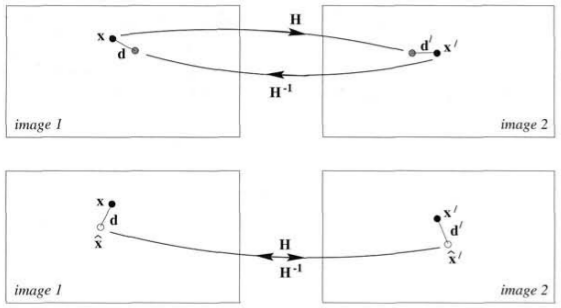
\includegraphics[width=6cm,natwidth=561,natheight=308]{figs/errors.png}
\label{fig:p1}
\end{figure}
\item Normalización:
Proceso realizado sobre los puntos antes de ejecutar DLT ya que éste no es invariante
ante similaridades. Un pequeño cambio en la escala de los parámetros $w_i$ y $\hat{w}_i$
afecta significativamente el resultado.
El proceso consiste en:
\begin{itemize}
\item Encontrar un par de transformaciones $T$ y $T'$ tal que los puntos 
$x_i$ y $x_i'$ respectivamente queden trasladados de tal forma que su centroide
sea el origne y que su distancia promedio a este centroide sea
igual a $\sqrt{2}$.
\item Transformar las coordenadas de la imágen según las transformaciones 
$T$ y $T'$ así: $\hat{x}_i'=Tx_i$ y $\hat{x}_i'=T'x_i'$
\end{itemize} 
Luego de estos pasos, los datos quedan normalizados y se procede a encontrar 
la $\hat{H}$ con DLT, donde:
\begin{equation*}
\begin{aligned}
x_i'&=Hx_i \\
T^{'-1}\hat{x}_i' &= H T^{-1}\hat{x}_i\\
\hat{x}_i'&= \underbrace{T'HT^{-1}}_\text{$\hat{H}$}\hat{x}_i
\end{aligned}
\end{equation*}
Luego de encontrar $\hat{H}$ se procede a desnormalizar mediante
\begin{equation*}
\begin{aligned}
H = T^{'-1}\hat{H}T
\end{aligned}
\end{equation*} 
\end{enumerate} 

\nocite{hartley2000multiple}
\bibliographystyle{plain}
\bibliography{biblio}

\end{document}
